\section{Agile software development}
\begin{table}[H]
\caption{diff. between plan-driven and agile}
Pland-driven: \newline
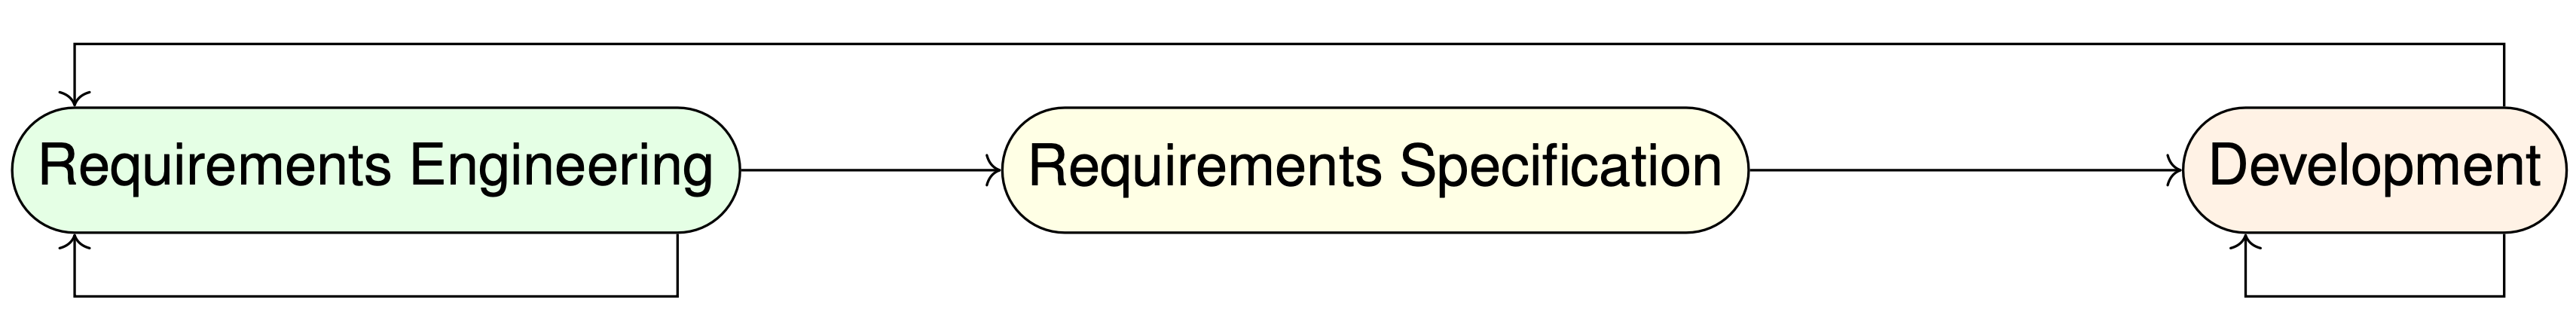
\includegraphics[scale=0.125]{plan_driven.png}
Agile: \newline
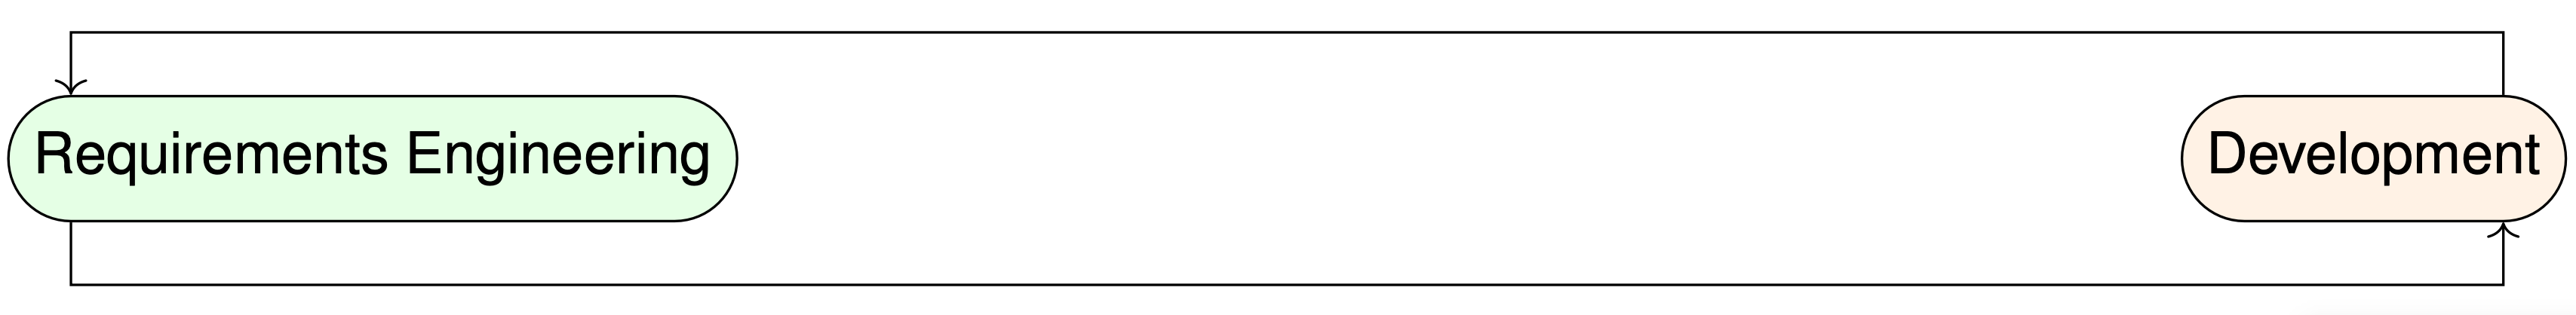
\includegraphics[scale=0.125]{agile.png}
\end{table}
$\bold{Agile}$ $\bold{manifesto}$:
\begin{enumerate}
	\item Individuen und Interaktionen über Prozessen und Werkzeugen
	\item Funktionierende Software über akribischer Dokumentation
	\item Zusammenarbeit mit dem Kunden über Vertragsverhandlungen
	\item Auf Veränderungen eingehen über Plan folgen
\end{enumerate}
\begin{table}[H]
\caption{Generic model}
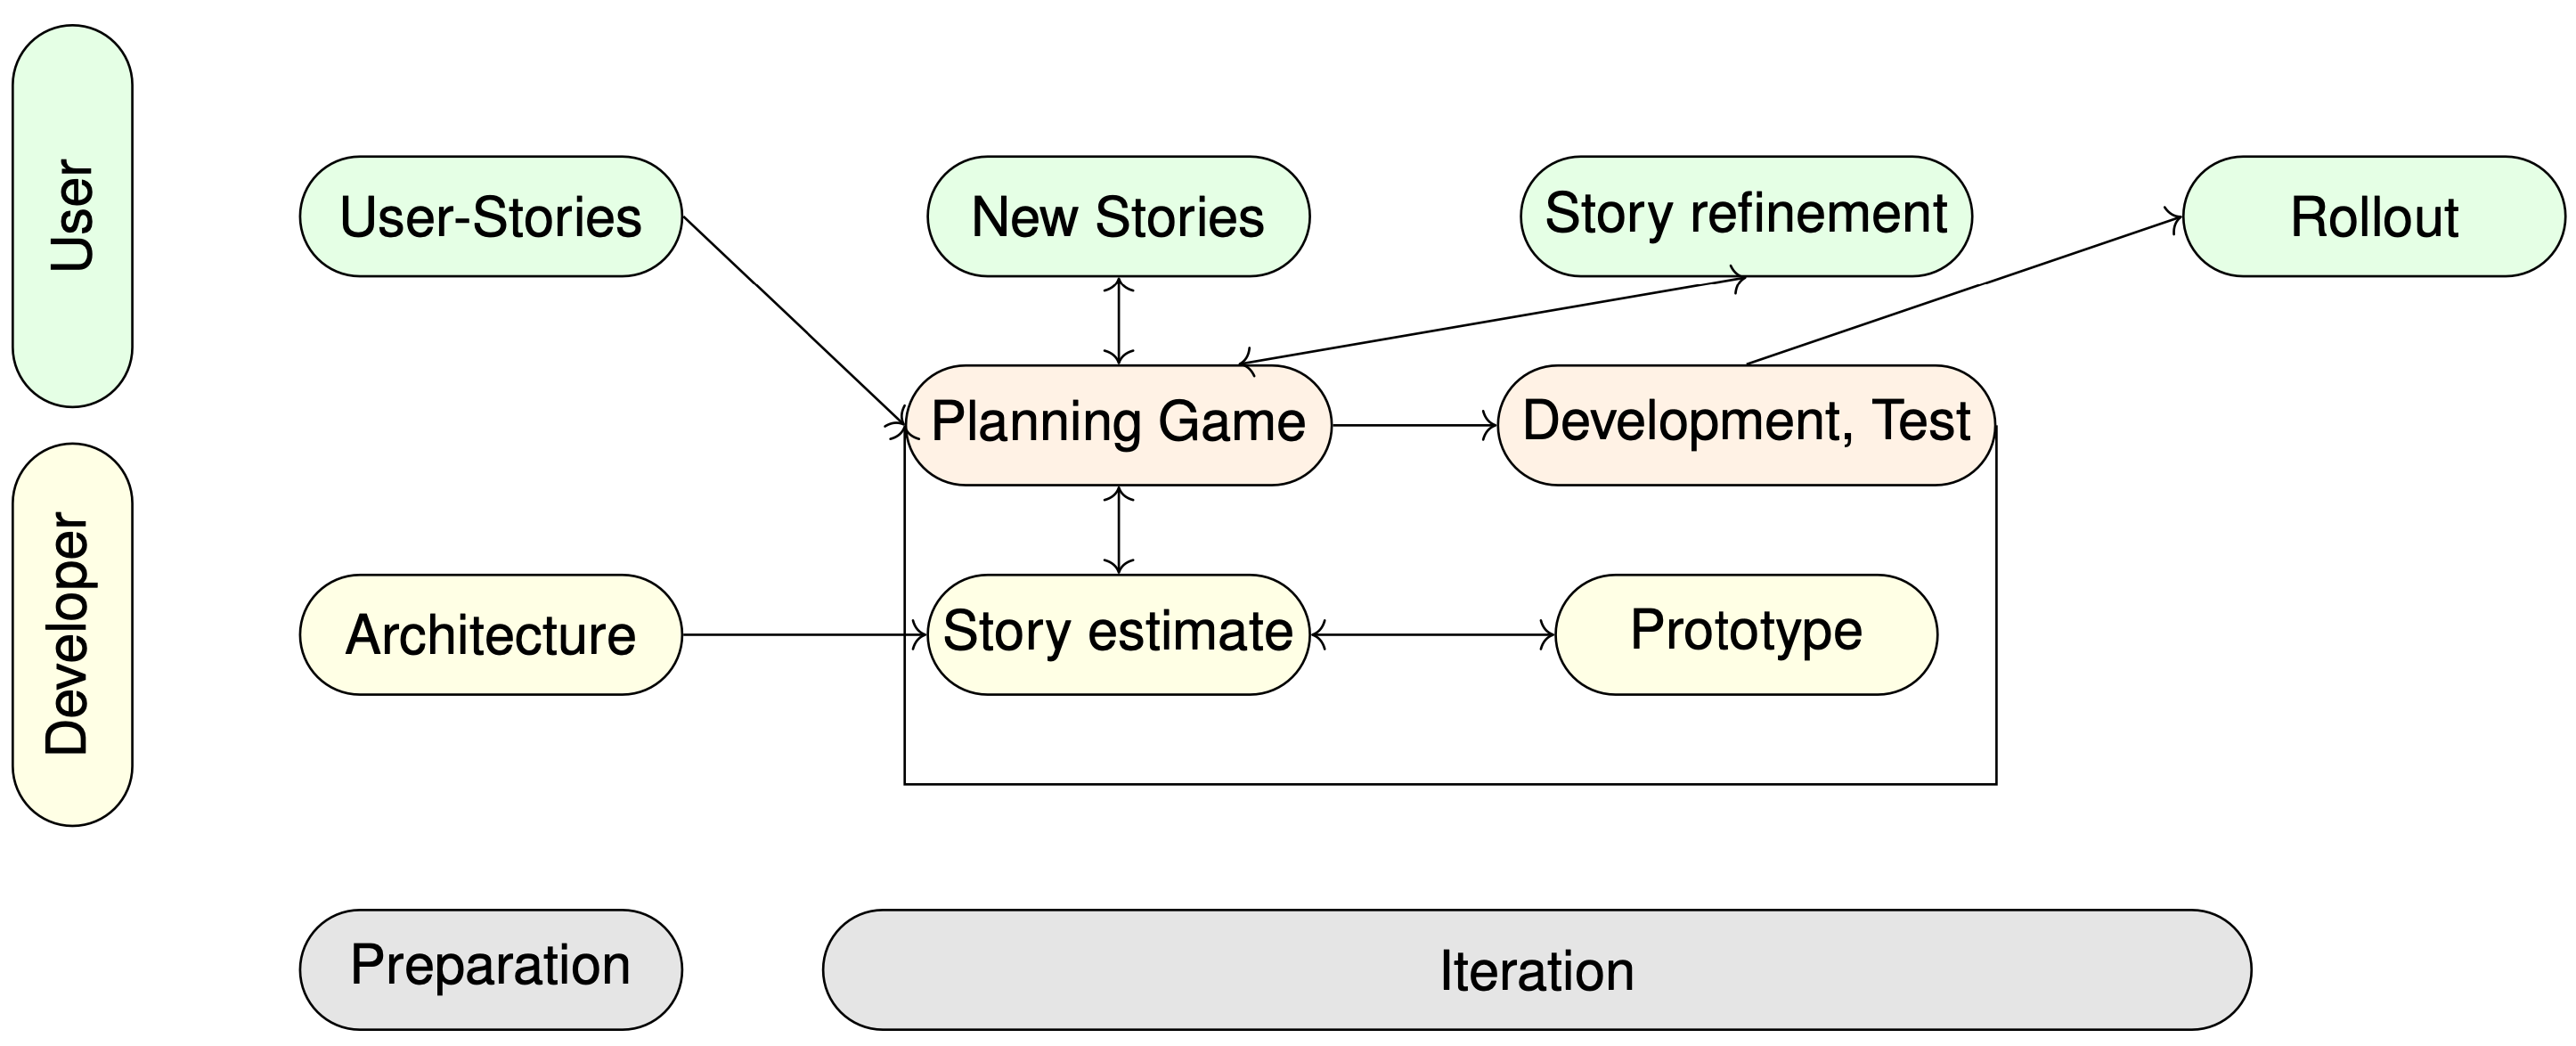
\includegraphics[scale=0.125]{generic_model.png}
\end{table}